%pdflatex-../thesis.tex
% vim:spell spelllang=en_us

Themis is an application for evaluation of virtual machine migrations. It is prepared to be used for availability measurements and can be easily adjusted to perform other task during migration. 

Application is modular and can be adapted for different orchestrator than OpenNebula. Architecture is depicted in figure \ref{img:themis-model}. Backend is responsible for measurement management and processing the results. Frontend provides web interface. Result can be displayed directly as table or graph in browser or exported in \Ac{CSV} format.

\begin{figure}[htb]
	\begin{center}
	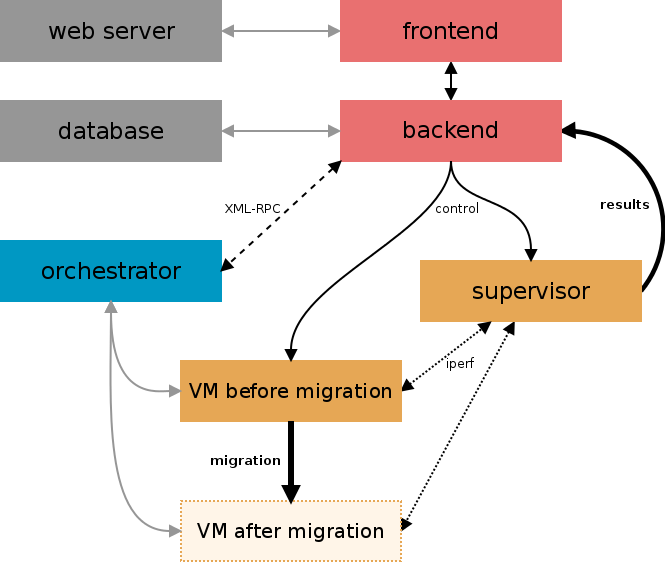
\includegraphics[width=0.7\textwidth]{themis-model.png}
	\end{center}
	\caption{Architecture of Themis application}
	\label{img:themis-model}
\end{figure}

% languages
Application is written in Ruby using Ruby on Rails framework. Ruby is platform independent and can run on almost every currently used operating system. Ruby on Rails (\Ac{RoR}) is framework providing database abstraction and it is strictly based on model-view-controller (\Ac{MVC}) architecture. Application defined by an object model, outputs are generatied using views and controller is responsible for sending commands to models and forward results to views.

I have decided to use this framework because it provides better interaction with system services, e.g. \Ac{SSH} and \Ac{SCP}, than other web frameworks. There are public available classes for interaction with OpenNebula and OpenStack cloud \Ac{API} so it is not necessary to create \mbox{\Ac{XML}-\Ac{RPC}} parsers from scratch.

\section{Measure models}
There are three models of measurement tasks and results. It is definition, session and transfer. These models are used to describe migration tasks instructions, migration progress and results. 
Relation between models is depicted in the figure \ref{img:themis-models-brief}.

All measurement models mentioned bellow are descendants of an \Name{ActiveRecord::Base} and mapping between objects and tables is handled by this build-in class. It also describes inter-model associations and performs validation. 

\begin{figure}[htb]
	\begin{center}
	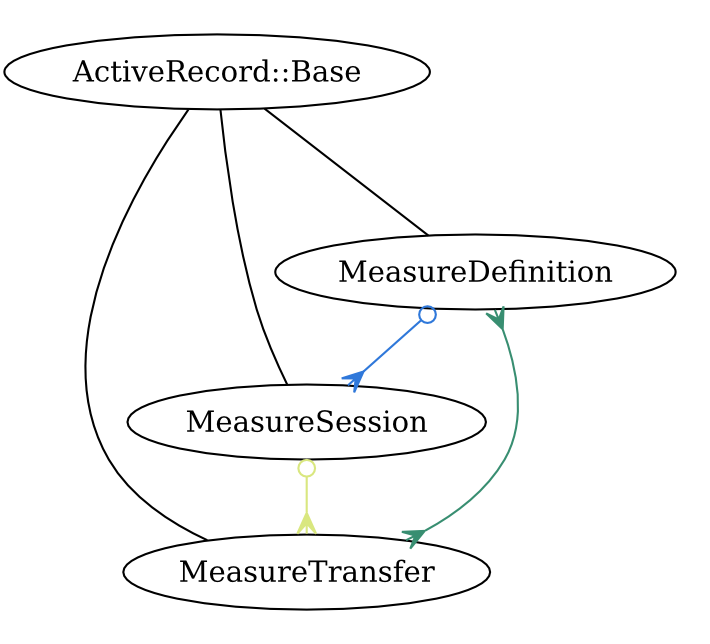
\includegraphics[width=0.6\textwidth]{models_brief.png}
	\end{center}
	\caption{Relation between measurement models}
	\label{img:themis-models-brief}
\end{figure}


\subsection{Definition}
Definition class, formally MeasureDefinition, is used to save prescription for measurement task and track time taken. Parameters are listed in the table \ref{tab:measuredefinition-params} and their meaning is described bellow.

\begin{description}
	\item[vm] is virtual machine which is going to be migrated. List of \Ac{VM}s available for migration is loaded on-demand from orchestrator using OneOrchestrator class. Virtual machine must be in running state and variable \Code{THEMIS\_TYPE = 'VM'} need to be present in contextualization settings.
	\item[source] is source host for virtual machine. \Ac{VM} need to be migrated to this host before starting measurement session. List of hosts is loaded using OneOrchestrator class and hosts status is checked for each host.
	\item[destination] is destination host. \Ac{VM} is migrated to this host during measurement session.
	\item[bandwidth] determines packet generation rate passed to the agent.
	\item[cycles] set number of migration repetitions.
	\item[supervisor] is an \Ac{IP} address of supervisor services, i.e. packet receiver and result exporter
	\item[description] can by used to attach any note.

	\item[started\_at] is timestamp taken at the beginning of measurement.
	\item[finished\_at] is timestamp taken after finishing all migrations.
\end{description}

Definition class has one-to-many relation with session class and also one-to-many indirect relation with transfer class connected through sessions. It means that it is possible to load every information from subordinate classes (models) and it is useful for generating exports and web views.

Definition class is the highest class in the hierarchy so it is connected with orchestrator. There is a class variable {@@shared\_orchestrator} which is providing link to an orchestrator interface. This variable is shared by all class instances so it is not necessary to initialize more parallel connections.

Methods for manipulation with orchestrator resources are declared in definition class. \Name{Host\_source} and \Name{host\_destination} returns host object for source and destination host. Method called \Name{virtual\_machine} returns virtual machine object which is going be used for migration evaluation and control.

Most important method of the definition class is \Name{start} because it executes migration evaluation. It is responsible for generation of sessions and starting all of them. One session object will be prepared for each migration cycle, so number of session objects is the same as number stored in cycles parameter. Sessions need to be started one by one so there is an loop which starts new session right after finishing the previous one. Session start is performed by calling \Name{start} of session class. This method is different from previously mentioned method with same name because this one is defined in session class.
Finished\_at parameter is set to current timestamp right after finishing of last session, i.e. at the end of migration evaluation. 

Migration evaluation is not very computation expensive, but it can take really long time to perform many migration cycles, in particular for virtual machines under load. It is not possible to run these long running tasks on request from web interface because request will timeout shortly and task would be terminated. I have decided to use Delayed::Job (\Ac{DJ}) to run these task asynchronously.
\Ac{DJ} can run task in detached process and it can run for a long time without any timeout problems. It is also possible to run \Ac{DJ} worker on separate machine so migration evaluation is executed in completely separated environment. This approach eliminates interference with other processes or network traffic. Security is improved too, since the orchestrator interface does not need to be accessible from machine serving web interface.

There is one special function called flush and it clears measurement definition and all of it's subordinate objects. It can be used for debugging because it is sometimes necessary to repeat the migration with same parameters. However it is not possible to run migration which was running in the past and all of sessions have already finished.

\begin{table}[htb]
\begin{center}
	\caption{MeasureDefinition parameters}

	\label{tab:measuredefinition-params}
	\begin{tabular}{|l|l|l|l|l|}
	\hline
	\Th{Parameter} & \Th{Required} & \Th{Type} & \Th{Editable by user} & \Th{Notes} \\
	\hline
	vm & yes & string & yes & \\
	\hline
	source & yes & integer & yes & \\
	\hline
	destination & yes & integer & yes & \\
	\hline
	bandwidth & yes & integer & yes & \\
	\hline
	cycles & yes & integer & yes & required bigger than 0\\
	\hline
	supervisor & yes & string & yes & \Ac{IP} address \\ 
	\hline
	description & no & text & yes & \\
	\hline
	started\_at & no & timestamp & no & \\
	\hline
	finished\_at & no & timestamp & no & \\
	\hline
	\end{tabular}
\end{center}
\end{table}


\subsection{Session}
Session class, precisely MeasureSession, is a link between definition and transfers. This class is responsible for migration and measurement coordination. Remote management of virtual machines and orchestrator is performed inside this class.

There are no parameters editable by a user because all necessary information about migration are inherited from the definition. Table \ref{tab:measuresession-params} describes all parameters. There are two timestamp fields with evident purpose, reference to MeasureDefinition and two fields special for this class:
\begin{description}
	\item[seq] is sequence number in scope of superior MeasureDefinition. Session with \mbox{$\mathrm{seq} = 1$} is going to be executed first and $\mathrm{seq} = \mathrm{measure\_definition.cycles}$ is the last one.
	\item[status] determines status of measurement session:
		\begin{itemize}
			\item \B{0} - pending - session is waiting for execution, this is the default state
			\item \B{1} - running - session is running right now
			\item \B{2} - done - migration was finished successfully
			\item \B{3} - failed - migration was executed and failed to finish
		\end{itemize}
\end{description}

\begin{table}[htb]
\begin{center}
	\caption{MeasureSession parameters}
	\label{tab:measuresession-params}
	\begin{tabularx}{\textwidth}{|l|l|l|l|X|}
	\hline
	\Th{Parameter} & \Th{Required} & \Th{Type} & \Th{Edit.} & \Th{Notes} \\
	\hline
	measure\_definition\_id & yes & reference & no & reference to MeasureDefinition \\
	\hline
	status & yes & integer & no & \\ 
	\hline
	seq & yes & integer & no & \\
	\hline
	started\_at & no & timestamp & no & \\
	\hline
	finished\_at & no & timestamp & no & \\
	\hline
	\end{tabularx}
\end{center}
\end{table}


Most important part of MeasureSession class is \Name{start} method. This method is executed by superior definition, so it is not necessary to set an asynchronous execution with Delayed::Job because higher object is already running asynchronously.

It is necessary to load migration parameters, so only an information about supervisor \Ac{IP} is loaded as a string and the rest is loaded as objects. It is beneficial to work with objects instead of identifiers because it allows to execute commands directly without any additional parsing.

Net::SSH client library is used for connection to virtual machine under test and supervisor. I have implemented authentication using keys because it is necessary to provide password-less login for the backend service. It is possible to implement password authentication just by editing the client library configuration, but I wanted to avoid storing any passwords in the source code. 

Migration process can be divided into 3 stages. First stage is preparation for migration, second stage is migration and third stage is migration verification and reporting. Tasks must be carried out sequentially because next task always depends on previous one.

First task after loading migration information is clearing previous measurement session. Established session between packet generator and packer receiver can become stale if it was not terminated successfully after previous migration. Packet generator and receiver should be terminated after virtual machine migration, but it may stay running in case of unexpected backend error or unclean shutdown. Command in the figure \ref{cmd:killcmd} is executed on \Ac{VM} and supervisor just to be sure there are no stale sessions. This command is optimized for agent.rb and need to be adapted to work with another measurement tools.

\begin{figure}[htb]
\caption{Clear stale sessions command}
\label{cmd:killcmd}
\begin{verbatim}
KILLPID=$(ps aux | grep -v grep | grep agent\.rb | grep ruby \
| xargs | cut -d' ' -f2); if [ -n "$KILLPID" ]; then \
kill -SIGINT "$KILLPID"; fi 
\end{verbatim}
\end{figure}

Next action performed during the first stage is migration to the source host. Source and destination hosts are loaded from the measure definition and the migration must be performed exactly from the source to the destination, so the \Ac{VM} need to be running on the source host. Unmeasured migration to source host is requested during this stage if \Ac{VM} is not already running on right host.

Last task in preparation stage is to run agents. It is necessary to start agents on \Ac{VM} and supervisor. Both agents must stay running after \Ac{SSH} disconnection. It is a bit tricky to run a Ruby script on a remote machine in a subshell because normal behavior it is to terminate process after disconnection. I am using \Cmd{screen} software which is able to run detached processes. However situation is even more complicated due to different Ruby installation methods on \Ac{VM} and supervisor. Virtual machine uses standard Ruby version installed via package manager by command \Cmd{apt-get install ruby}, so it easier to run agent.rb because it does not require interactive shell. Rbenv\footnote{\url{https://github.com/sstephenson/rbenv}} is used to install Ruby on supervisor because agent.rb in receiver mode requires newer version than provided by package manager. Rbenv is initialized in file \~/.bashrc so it is necessary to run all Ruby scripts in interactive shell. Parameters for agent.rb can be found below in the table \ref{tab:agent-parameters}.

\begin{figure}[htb]
\caption{Run remote agents command}
\label{cmd:remote agents}
\begin{verbatim}
###  generator - VM
screen -d -m /bin/bash -c '~/themis/agent.rb "generator" \
#{supervisor} #{5000 + (id % 1000)} #{measure_definition.bandwidth}M'

### receiver - supervisor
screen -d -m /bin/bash -li -c '~/themis/agent.rb "receiver" \
#{supervisor} #{5000 + (id % 1000)} \
#{measure_transfers_upload_url(:measure_session => id, :format => 'json')}'
\end{verbatim}
\end{figure}

\subsubsection{Known problems}

Sessions are not atomic because asynchronous \Ac{API} is used and many sequential actions need to be performed. Orchestrator works in \Uv{best effort} manner, so migration request is refused sometimes. It is usually caused by temporary unknown \Ac{VM} state. This behavior can not be solved in application so this kind of session is just marked as failed and next session is started. 

Another problem is virtual machine stuck in migration state. It is caused by hypervisor error (usually deadlock). Orchestrator keeps asking about virtual machine state but never gets an answer, so virtual machine is stuck in actual state. It is necessary to fix this error manually in orchestrator because application will get stuck in waiting for migration to finish. It is necessary to fix faulty hypervisor, delete \Ac{VM} and recreate it.
Measurement task will continue after \Ac{VM} under test is back in running state.

Most serious problem is caused by zombie \Ac{VM}s. Zombie is virtual machine running on hypervisor, although it should not. Even worse is that OpenNebula orchestrator does not display zombies in list of virtual machines and it is possible to deploy virtual machine with same id on different host. This situation is depicted in figure \ref{img:themis-zombie}. It is obviously not possible to migrate \Name{one-247} between hosts because it already exists on both of them. I am working on modification of OpenNebula scheduler to stop deployment of virtual machine in case of zombie with same name already exists.

\begin{figure}[htb]
	\begin{center}
	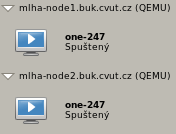
\includegraphics[scale=0.8]{zombie.png}
	\end{center}
	\caption{Zombie \Ac{VM}}
	\label{img:themis-zombie}
\end{figure}

All of these errors are cause by incorrect orchestrator behavior, so it is necessary to solve them in orchestrator. Application will wait for problem to be fixed or labels session as failed.



\subsection{Transfer}
Class MeasureTransfer is used to store information about the transfers and it is actually parsed output from packet receiver. There are no user editable fields because objects are uploaded via \Ac{API}. Model parameters are described in the table \ref{tab:measuretransfer-params}.

Themis application use iperf to measure packet flow, so MeasureTransfer class is tailored for output of the iperf. Adapting to another measurement software is fairly easy because just one database migration script and small model changes will do the job.

\begin{table}[htb]
\begin{center}
	\caption{MeasureTransfer parameters}
	\label{tab:measuretransfer-params}
	\begin{tabularx}{\textwidth}{|l|l|l|l|X|}
	\hline
	\Th{Parameter} & \Th{Required} & \Th{Type} & \Th{Edit.} & \Th{Notes} \\
	\hline
	measure\_session\_id & yes & reference & no & reference to MeasureSession \\
	\hline
	timestamp & no & timestamp & no & \\
	\hline
	time\_relative & yes & float & no & \\
	\hline
	jitter & no & float & no & \\
	\hline
	datagrams\_transfered & no & integer & no & \\
	\hline
	datagrams\_lost & no & integer & no & \\
	\hline
	bits\_transfered & no & integer & no & \\
	\hline
	bits\_lost & no & integer & no & \\
	\hline
	bandwidth & no & integer & no & bits per second\\
	\hline
	\end{tabularx}
\end{center}
\end{table}

I it necessary to provide interface for automatic uploading MeasureTransfer objects. \Ac{URL} for uploads is /measure\_transfers/:measure\_session(.:format) and it is routed to measure\_transfers\#upload. This \Ac{URL} needs to be passed to the packet generator. 

First task is to load the superior MeasureSession object and check whether this object actually exists. Transfers without a session is not valid and can no be saved.

Upload action of MeasureTranfers controller parses input objects received in \Ac{JSON} format and saves them into the database. However it is necessary to make a few changes to each object. Iperf uses different format of timestamp than database and it does not support time zone, so each timestamp received from the iperf must be parsed, converted to native DateTime object and merged with timezone data. 

Parsed DateTime object is used to calculate time\_relative. It is time between current time and start of migration session. Relative time is used to align migrations for graphing and exports.

Rails framework implements \Ac{CSRF} prevention mechanism, so it is necessary to create an exception for an upload action. I have added exception to ApplicationController for all request in the \Ac{JSON} format.


\section{Virtual machines}
Virtual machine, used for migration testing, needs to be prepared first. It is possible to migrate every virtual machine, but agent.rb wrapper needs. Agent is also used to export results from the supervisor to the backend.

Agent.rb is expected to exist in path {\~/themis/agent.rb} and it is already saved there in prepared images. It is also necessary to install Ruby interpreter. I have used package available in distribution for \Ac{VM} under test and rbenv for supervisor.

Virtual machines are save on attached CD. Both are already contextualized for OpenNebula, and agent.rb with Ruby is installed. These images can be directly imported into OpenNebula image datastore and used in templates.

\begin{table}[htb]
\begin{center}
	\caption{Virtual machines parameters}
	\label{tab:vm-params}
	\begin{tabular}{|l|l|l|}
	\hline
	\Th{Parameter} & \Th{VM for migration} & \Th{Supervisor} \\
	\hline
	Operating system & \multicolumn{2}{c|}{Ubuntu server 14.04.1 LTS} \\
	\hline
	Kernel version & \multicolumn{2}{c|}{3.13.0-32} \\
	\hline
	Image size & \multicolumn{2}{c|}{5.9G} \\
	\hline
	Image type & \multicolumn{2}{c|}{raw} \\
	\hline
	Device prefix & \multicolumn{2}{c|}{vd} \\
	\hline
	Username & \multicolumn{2}{c|}{root} \\
	\hline
	Password & \multicolumn{2}{c|}{none, only \Ac{SSH} keys using contextualization}\\
	\hline
	Agent.rb & \multicolumn{2}{c|}{/root/themis/agent.rb}\\
	\hline
	Ruby version & 1.9.3p484 & 2.1.3p242 \\
	\hline
	Ruby install method & package manager & rbenv \\
	%\hline - image changed - it is necessary to recount hash
	%MD5 hash & 285a5...77a9f8e68bf0cc & 8cf08...83511ce9857a4 \\
	\hline
	\end{tabular}
\end{center}
\end{table}


\section{Agent}
It was necessary to develop a script wrapper capable to parse iperf output and upload results to the backend module. This script is called agent.rb, it is attached on on the CD and will be published in project repository. It is written in Ruby to be compatible with the rest of the project. Agent script is executed by thby thee backend in migration\_session model in start method and \Ac{SSH} is used for remote execution.

Agent script needs to be available in the virtual machine under test as well as in supervisor. However distribution is fairly simple because it is just a single file (agent.rb) with a few dependencies. This file can be distributed manually, but it is not very usable for large or frequent deployment. Automatic deployment using OpenNebula's contextualization is much more efficient since orchestrator takes care of saving file into \Ac{VM}s. 
It is also possible to use configuration management system to upload this file and prepare environment to run migration. I am using Ansible to deploy agent.rb because it was necessary to update Ruby version. 

There are two modes of running agent. Modes differ in packet generator parameters and required dependencies. Mode is determined by \Code{ARGV[0]} parameter, which is the first parameter after filename. It is necessary to select correct mode and properly configure all parameters from the table \ref{tab:agent-parameters} because measure session can not be established otherwise. 

Generator mode only creates packets and sends them to receiver so it requires nothing more than the Ruby and the iperf available. Receiver mode is more advanced and it uploads results to the backend besides receiving packets. Receiver mode requires these dependencies:
\begin{itemize}
	\item \B{net/http} used to upload results to then backend using \Ac{HTTP} POST method
	\item \B{json} necessary to export data into \Ac{JSON} before sending
	\item \B{date} used to parse iperf timestamp and convert it into backend compatible format
\end{itemize}

% dependencies 
Both modes use IO class to read pipeline output from iperf program. This class is part of a Ruby core so it is not necessary to install it separately. Receiver dependencies can be installed using package manager or with gem utility using command \Cmd{gem install net/http json date}.

\begin{table}[htb]
\begin{center}
	\caption{Agent.rb parameters}
	\label{tab:agent-parameters}
	\begin{tabularx}{\textwidth}{|r|l|l||l|X|}
	\multicolumn{3}{c}{\Th{Generator mode}} & \multicolumn{2}{c}{\Th{Receiver mode}} \\
	\hline
	\Code{ARGV[i]} & {Parameter} & {Example}  & {Parameter} & {Example} \\
	\hline
	\hline
	0 & Mode & generator & Mode & receiver \\
	\hline
	1 & Destination \Ac{IP} & 192.0.2.1 & Listen \Ac{IP} & 192.0.2.1 \\
	\hline
	2 & Destination port & 5004 & Listen port & 5004 \\
	\hline
	3 & Bandwidth & 1M & Upload \Ac{URL} & \url{http://backend/measure_transfers/23.json} \\
	\hline
	\end{tabularx}
\end{center}
\end{table}


% iperf crap
Agent is using legacy iperf version developed by NLANR/DAST, but it introduces several problems which must be resolved in agent.rb and measure session routine. I am going to adapt agent.rb for iperf3\footnote{Available on \url{https://github.com/esnet/iperf}}. It is a new implementation developed by ESnet/Lawrence Berkeley National Laboratory. Iperf3 provides \Ac{JSON} output and probably will not suffer from problems presented below.

First problem is automatic session reestablishment. This occurs when running session is interrupted by a client and new session is initialized with the same receiver in short interval (less than few seconds). Iperf server joins new session with previous one which is not desired solution. This it the reason why there is 5 second interval inserted before generator restart. 

Second problem is handling INT signal by legacy iperf. SIGINT is reserved for external interrupt and this signal is, for example, sent to process when \mbox{Ctrl + C} is pressed. Iperf catches this signal preventing user to accidentally stop running measure session. I understand reason why this function was implemented but I think that is total nonsense to require two consecutive INT signals to quit program. I have solved this by trapping SIGINT and sending KILL signal to iperf before agent.rb exits. This is only one possible way to reliably stop running agent together with the iperf.

\begin{figure}[htb]
\caption{Example of agent.rb and iperf commands}
\label{code:fw}
\begin{verbatim}
# agent in generator mode
./agent.rb "generator" 192.0.2.1 5004 10M
# expanded iperf command in generator mode
iperf --udp --interval 1 --time 3600 --client 192.0.2.1 --port 5004 \
--bandwidth 10M --format b
	
# agent in receiver mode
./agent.rb "receiver" 192.0.2.1 5004 http://backend/measure_transfers/23.json
# expanded iperf command in receiver mode
iperf --server --bind 192.0.2.1 --port 5004 --udp --interval \
--reportstyle c --format
\end{verbatim}
\end{figure}



\section{Frontend}
I have developed web interface for managing Themis application because it is easier for users to interact with web interface then configure application using console. Although web interface was not main goal of this thesis, I have decided to implement it to provide better information about running migration and simple interface.

Web frontend is created in respect with model-view-architecture of Ruby on Rails. Twitter Bootstrap\footnote{\url{https://github.com/twbs/bootstrap}} is used for user interface components.

There are three tabs in the main page:
	\begin{itemize}
		\item Themis
		\item Waiting jobs
		\item Measure definitions
	\end{itemize}

First tab is just welcome page with elementary information. The most important information on this page is current version. Application is prepared to be deployed using Capistrano\footnote{\url{https://github.com/capistrano/capistrano}} so current running version is loaded from GIT repository.

Waiting jobs tab displays running and pending tasks. All long-running tasks need to be executed asynchronously with Delayed::Job, so task is first saved into the database and then executed by a worker after some time defined in the configuration. Pending and running jobs can be reviewed in this tab. However it is not allowed to perform any changes on running or pending task because it could break relation between Delayed::Job and running processes.

\subsection{Definitions}
Most important tab is Measure definitions because actions can be performed here. List of all definitions is displayed after clicking the tab, screenshot is in the figure \ref{img:themis-definitions}. User accessible parameters from table \ref{tab:measuredefinition-params} are displayed here. There are also basic actions as view, edit and destroy. Already started definition can not be edited.

\begin{figure}[htb]
	\begin{center}
	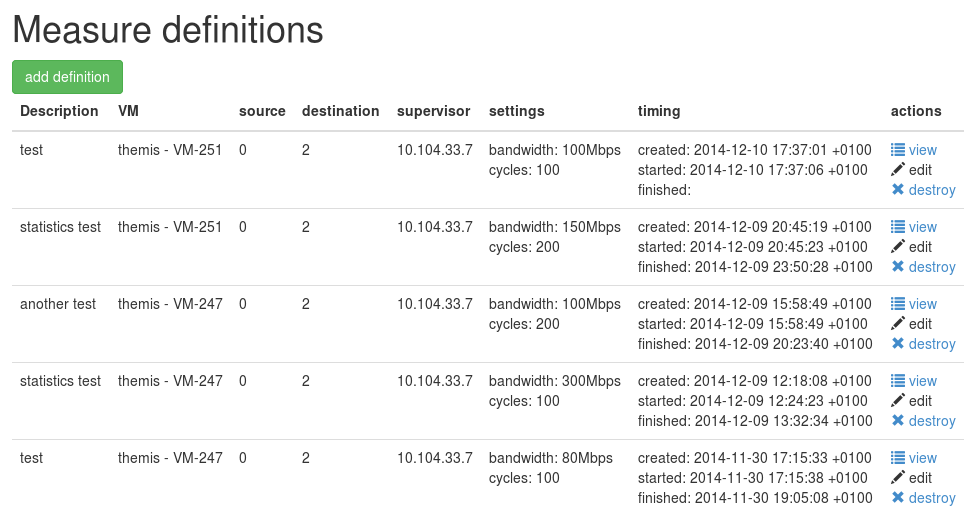
\includegraphics[width=\textwidth]{themis-definitions.png}
	\end{center}
	\caption{List of all definitions}
	\label{img:themis-definitions}
\end{figure}

I have decided to print source and destination host only as an id because each name lookup takes one request send to the orchestrator. I think that listing id is sufficient because user should already be familiar with OpenNebula hosts. 

More information about definition can be displayed by following \Uv{view} action link on the right side. This page displays all information about selected definition, it's parameters, sessions and transfers. Screenshot is in the figure \ref{img:themis-definition}.

\begin{figure}[htb]
	\begin{center}
	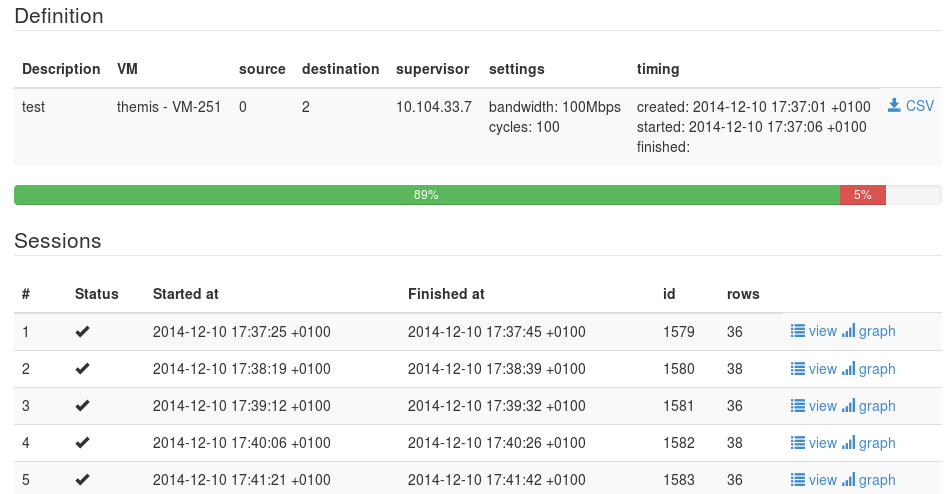
\includegraphics[width=\textwidth]{themis-definition.png}
	\end{center}
	\caption{Definition overview}
	\label{img:themis-definition}
\end{figure}

Progress bar represents ratio between finished, failed and pending sessions. First green part is ratio of successfully finished sessions to all migrations, red part is ratio of failed sessions and the rest is percentage of pending. 

There is table of all sessions under the progress bar. Session means one migration from source host to destination host together with network measurement.
Status, time of start end finish, id and number of rows is displayed for each session.

Information about transfers during session can be displayed as a table or a graph. Graphing library is Chart.js\footnote{\url{https://github.com/nnnick/Chart.js}} so it is necessary to use browser with JavaScript and \Ac{HTML}5 support. It is much slower to generate graph in browser than using MATLAB because it is not optimized to work with huge datasets. Graphing in browser is intended to be used for quick overview and more complex visualization can be generated from exported \Ac{CSV} file using MATLAB or matplotlib.

\begin{figure}[htb]
	\begin{center}
	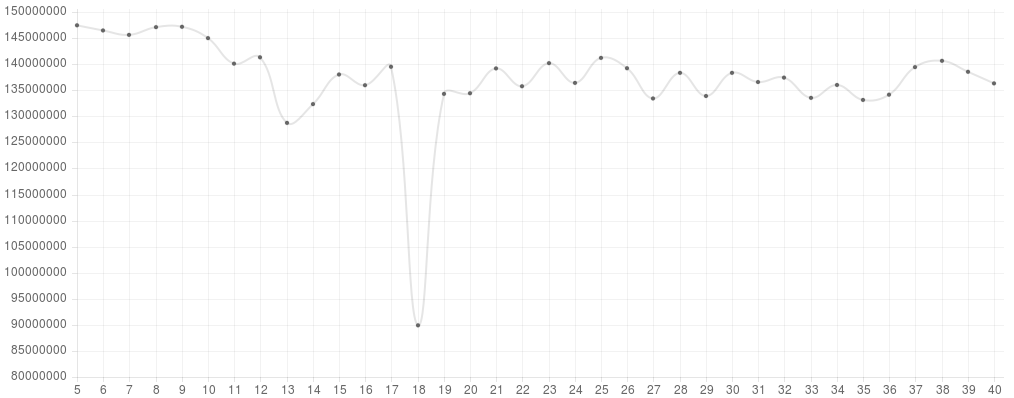
\includegraphics[width=\textwidth]{themis-graph-bw-1457.png}
	\end{center}
	\caption{Bandwidth visualization}
	\label{img:themis-graph}
\end{figure}

Frontend does not implement any kind of authorization and authentication because it is supposed to run on isolated network or as a part of existing system with authorization. Every client gets unlimited access to all migration data and can perform any action. It is necessary to negotiate rules in case of multiuser usage. It is not difficult to implement user access control, but it is beyond the scope of this thesis. Authentication library Authlogic\footnote{\url{https://github.com/binarylogic/authlogic}} can be uses with authorization provided by for example CanCanCan\footnote{\url{https://github.com/CanCanCommunity/cancancan}}.
